\documentclass[../body.tex]{subfiles}
\begin{document}
	\subsection{Гистограммы и графики плотности распределения}
	\begin{figure}[H]
		\centering
		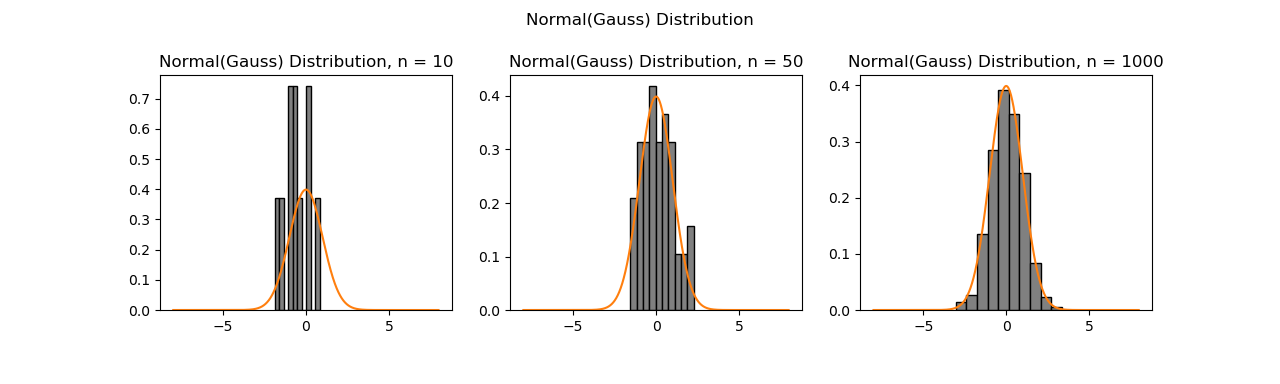
\includegraphics[width=\textwidth, height =0.25\textheight]{img/Normal.png}
		\caption{Нормальное распределение}
		\label{fig:normal}
	\end{figure}

	\begin{figure}[H]
		\centering
		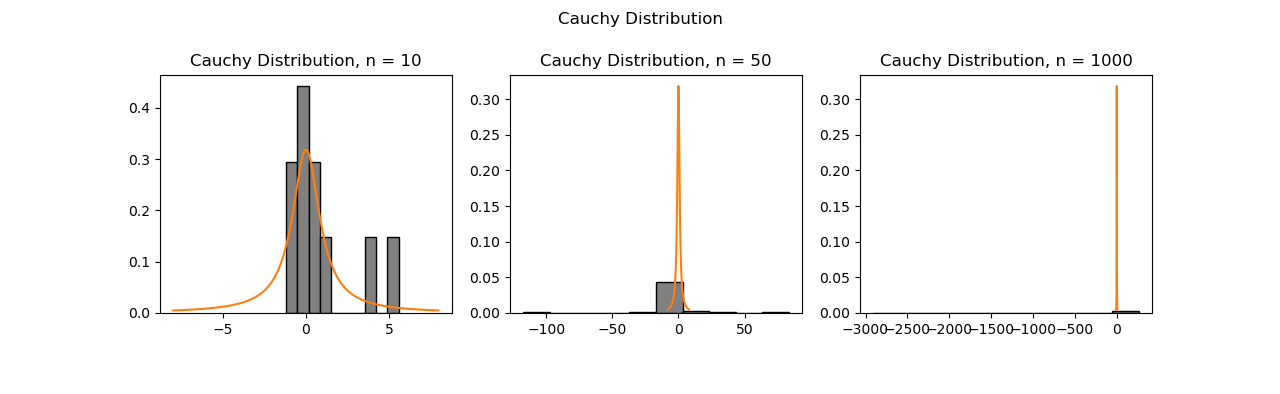
\includegraphics[width=\textwidth, height =0.25\textheight]{img/Cauchy.png}
		\caption{Распределение Коши}
		\label{fig:cauchy}
	\end{figure}
	

	\begin{figure}[H]
		\centering
		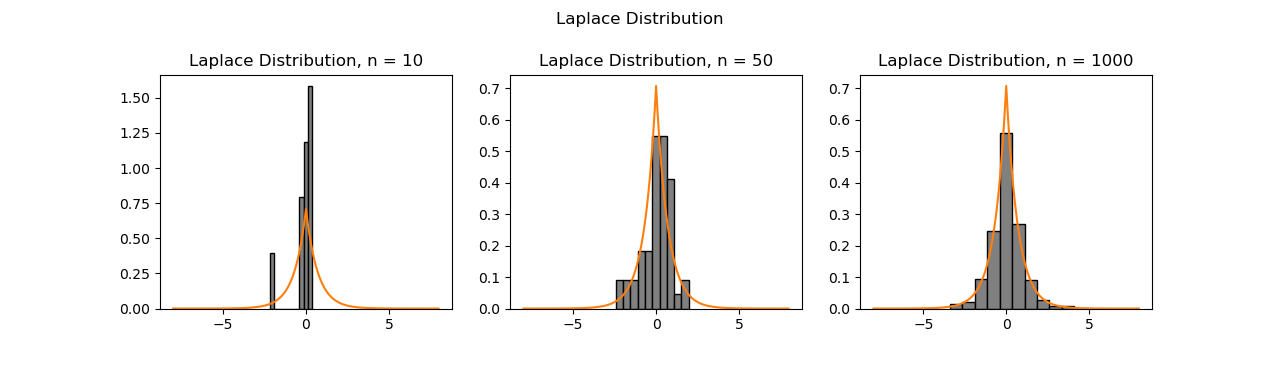
\includegraphics[width=\textwidth, height =0.25\textheight]{img/Laplace.png}
		\caption{Распределение Лапласа}
		\label{fig:laplace}
	\end{figure}


	\begin{figure}[H]
		\centering
		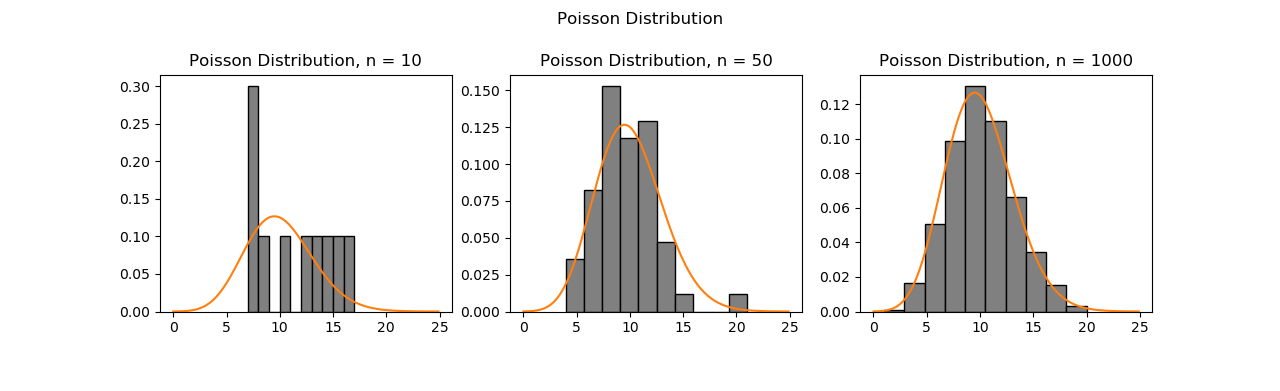
\includegraphics[width=\textwidth, height =0.25\textheight]{img/Poisson.png}
		\caption{Распределение Пуассона}
		\label{fig:poisson}
	\end{figure}


	\begin{figure}[H]
		\centering
		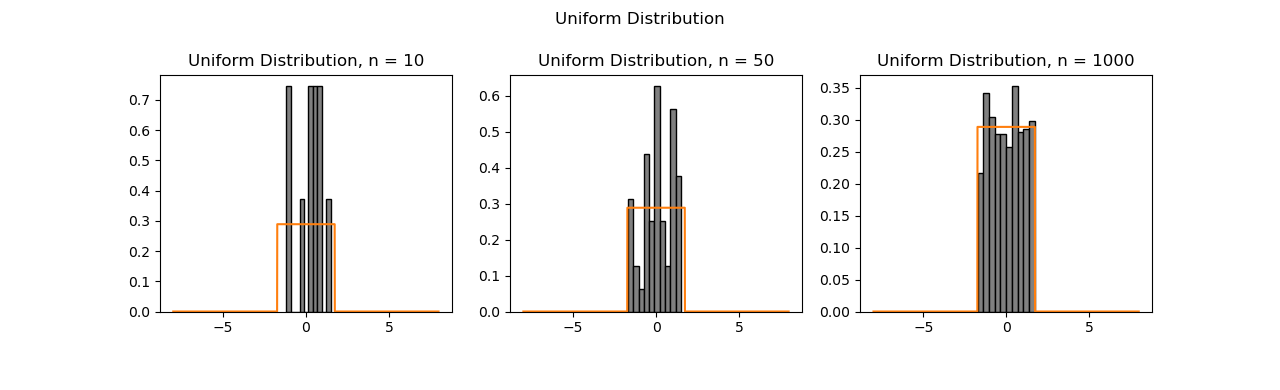
\includegraphics[width=\textwidth, height =0.25\textheight]{img/Uniform.png}
		\caption{Равномерное распределение}
		\label{fig:uniform}
	\end{figure}

	\subsection{Характеристики положения и рассеяния}
	Мощность выборки указана в первом столбике справа.
	\begin{table}[H]
		\centering
		\begin{tabular}[t]{lrrrrr}
			\hline
			Characteristic   &      Mean &    Median &       z\_R &      z\_Q &      z\_tr \\
			\hline
			Normal E(z) n = 10   &  0.00 &  0.0 &  0.0 & 0.0  &  0.0 \\
			Normal D(z) n = 10   &  0.099688 &  0.136509 &  0.189635 & 0.111227 &  0.110212 \\
			Normal E(z) n = 100  & -0.001 &  0.00  &  0.00 & 0.00 &  0.00 \\
			Normal D(z) n = 100  &  0.009908 &  0.01583  &  0.094601 & 0.012515 &  0.011928 \\
			Normal E(z) n = 1000 & -0.0001 & 0.000  & 0.00  & 0.000  & 0.000 \\
			Normal D(z) n = 1000 &  0.000974 &  0.001515 &  0.05807  & 0.001175 &  0.001128 \\
			\hline
		\end{tabular}
		\caption{Нормальное распределение}
		\label{tab:normal}
	\end{table}

	\begin{table}[H]
	\centering
		\begin{tabular}[t]{lrrrrr}
			\hline
			Characteristic   &        Mean &    Median &            z\_R &       z\_Q &      z\_tr \\
			\hline
			Cauchy E(z) n = 10   &   -0.6 &  0.0 &   -3.0     &  0.0 &  0.0 \\
			Cauchy D(z) n = 10   &  350.215    &  0.335402 & 8468.97        &  0.852087 &  0.491287 \\
			Cauchy E(z) n = 100  &   -2.1  & 0.00 & -104.000000       &  0.00 &  0.00 \\
			Cauchy D(z) n = 100  & 2224.86     &  0.023412 &    5.40494e+06 &  0.051584 &  0.02502  \\
			Cauchy E(z) n = 1000 &    1.0  &  0.000 &  511.00000000       &  0.000  &  0.000 \\
			Cauchy D(z) n = 1000 & 1195.76     &  0.002459 &    2.96612e+08 &  0.004937 &  0.002572 \\
			\hline
		\end{tabular}
	\caption{Распределение Коши}
	\label{tab:couchy}
	\end{table}
	
	\begin{table}[H]
	\centering
		\begin{tabular}[t]{lrrrrr}
			\hline
			Characteristic    &      Mean &    Median &       z\_R &       z\_Q &      z\_tr \\
			\hline
			Laplace E(z) n = 10   &  0.0 &  0.00 &  0.0 &  0.00 &  0.00 \\
			Laplace D(z) n = 10   &  0.109844 &  0.071526 &  0.473888 &  0.094274 &  0.075035 \\
			Laplace E(z) n = 100  &  0.00 &  0.001 &  0.0 &  0.00 & -0.002 \\
			Laplace D(z) n = 100  &  0.010475 &  0.005896 &  0.391706 &  0.010239 &  0.006378 \\
			Laplace E(z) n = 1000 &  0.0006 &  0.0001 &  0.0 &  0.0008 &  0.0006 \\
			Laplace D(z) n = 1000 &  0.000941 &  0.000479 &  0.386371 &  0.000996 &  0.000569 \\
			\hline
		\end{tabular}
		\caption{Распределение Лапласа}
		\label{tab:laplece}
	\end{table}

\begin{table}[H]
	\centering
	\begin{tabular}[t]{lrrrrr}
		\hline
		Characteristic    &      Mean &   Median &       z\_R &      z\_Q &     z\_tr \\
		\hline
		Poisson E(z) n = 10   & 10.00   & 9.8   & 10.30   & 9.9  & 9.8     \\
		Poisson D(z) n = 10   &  1.06412  & 1.44673  &  2.07481  & 1.23124  & 1.18912  \\
		Poisson E(z) n = 100  & 10.00   & 9.8   & 10.9    & 9.9  & 9.8   \\
		Poisson D(z) n = 100  &  0.098619 & 0.20429  &  0.940904 & 0.141224 & 0.119525 \\
		Poisson E(z) n = 1000 & 10.001   & 9.996    & 11.6    & 9.994  & 9.86  \\
		Poisson D(z) n = 1000 &  0.009728 & 0.003984 &  0.695475 & 0.002396 & 0.010941 \\
		\hline
	\end{tabular}
	
	\caption{Распределение Пуассона}
	\label{tab:poisson}
\end{table}

\begin{table}[H]
	\centering
	\begin{tabular}[t]{lrrrrr}
		\hline
		Characteristic    &      Mean &    Median &       z\_R &       z\_Q &      z\_tr \\
		\hline
		Uniform E(z) n = 10   &  0.01 &  0.0 &  0.01 &  0.0 &  0.0 \\
		Uniform D(z) n = 10   &  0.098933 &  0.223483 &  0.045204 &  0.141623 &  0.160647 \\
		Uniform E(z) n = 100  &  0.003 &  0.00 &  0.0001 &  0.00 &  0.00 \\
		Uniform D(z) n = 100  &  0.009705 &  0.029092 &  0.000589 &  0.013734 &  0.019446 \\
		Uniform E(z) n = 1000 &  0.000 &  0.002 & -5.1e-05  &  0.000 & -0.001   \\
		Uniform D(z) n = 1000 &  0.001027 &  0.003036 &  6e-06    &  0.001515 &  0.002039 \\
		\hline
	\end{tabular}
	\caption{Равномерное распределение}
	\label{tab:uniform}
\end{table}

\subsection{Боксплот Тьюки}
Для каждого распределения представлен боксплот Тьюки для выборок размером 20 и 100 элементов.
\begin{figure}[H]
	\centering
	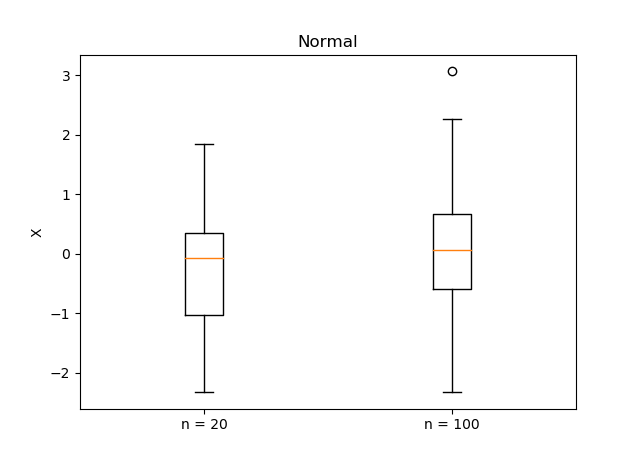
\includegraphics[width = 10cm, height = 8cm]{img/Normal_boxplot.png}
	\caption{Нормальное распределение}
	\label{fig:normal_boxplot}
\end{figure}

\begin{figure}[H]
	\centering
	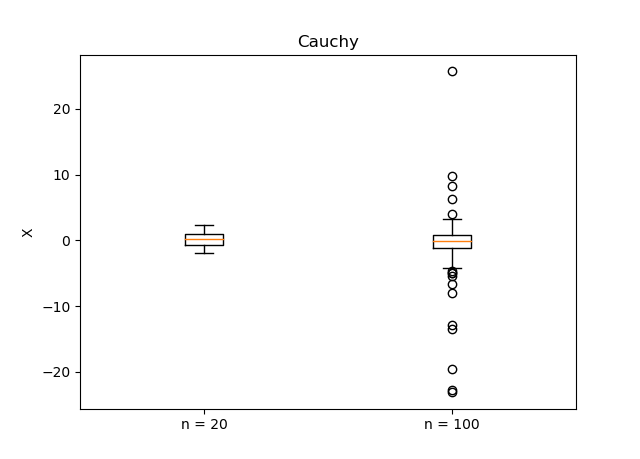
\includegraphics[width = 10cm, height = 8cm]{img/Cauchy_boxplot.png}
	\caption{Распределение Коши}
	\label{fig:cauchy_boxplot}
\end{figure}


\begin{figure}[H]
	\centering
	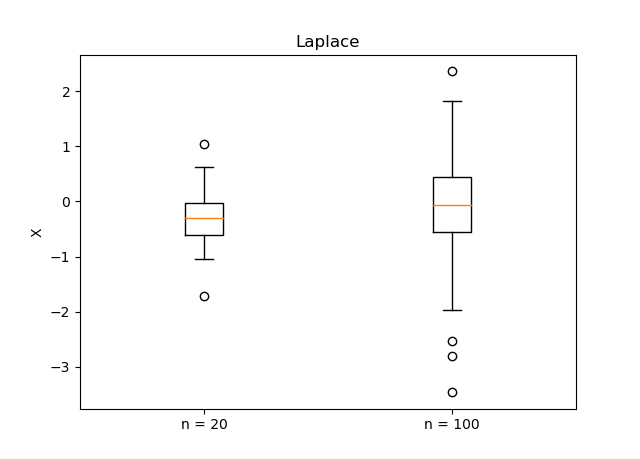
\includegraphics[width = 10cm, height = 8cm]{img/Laplace_boxplot.png}
	\caption{Распределение Лапласа}
	\label{fig:laplace_boxplot}
\end{figure}


\begin{figure}[H]
	\centering
	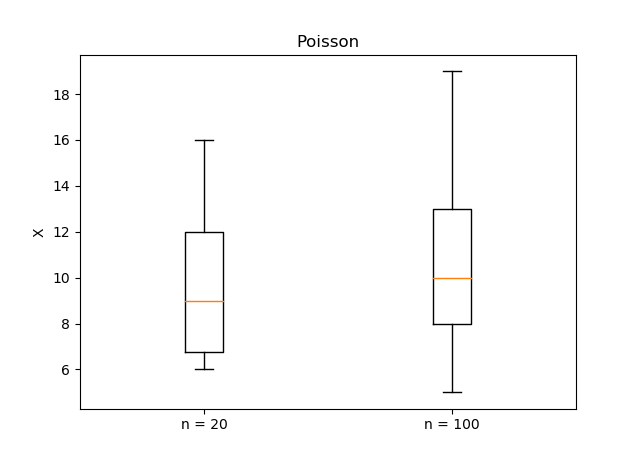
\includegraphics[width = 10cm, height = 8cm]{img/Poisson_boxplot.png}
	\caption{Распределение Пуассона}
	\label{fig:poisson_boxplot}
\end{figure}


\begin{figure}[H]
	\centering
	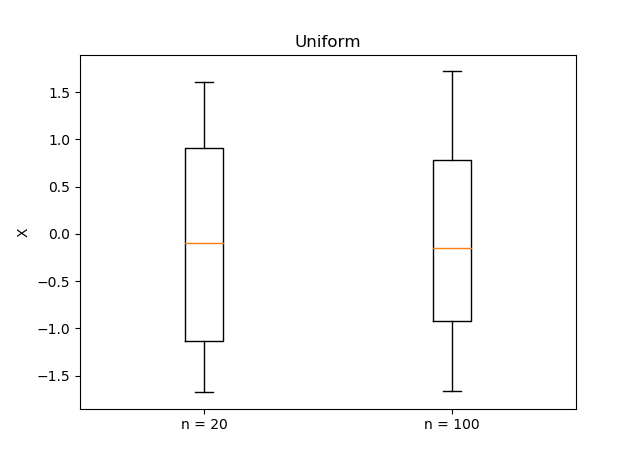
\includegraphics[width = 10cm, height = 8cm]{img/Uniform_boxplot.png}
	\caption{Равномерное распределение}
	\label{fig:uniform_boxplot}
\end{figure}

\subsection{Доля выбросов}
\begin{table}[H]
	\centering
	\begin{tabular}{lr}
		\hline
		Выборка          &   Доля выбросов \\
		\hline
		Normal, n = 20   &            0.02 \\
		Normal, n = 100  &            0.01 \\
		Cauchy, n = 20   &            0.15 \\
		Cauchy, n = 100  &            0.16 \\
		Laplace, n = 20  &            0.08 \\
		Laplace, n = 100 &            0.06 \\
		Poisson, n = 20  &            0.02 \\
		Poisson, n = 100 &            0.01 \\
		Uniform, n = 20  &            0    \\
		Uniform, n = 100 &            0    \\
		\hline
	\end{tabular}
	\caption{Доля выбросов}
	\label{tab:outliers}
\end{table}

\subsection{Теоретическая вероятность выбросов}
\begin{table}[H]
	\begin{center}
		\begin{tabular}{ l  c  c  c  c  c }
			\hline
			Распределение    & $Q_1^T$ & $Q_2^T$ & $X_1^T$ & $X_2^T$ & $P_B^T$ \\ \hline
			Нормальное распределение & -0.674 & 0.674 & -2.698 & 2.698 & 0.007 \\ 
			Распределение Коши & -1 & 1 & -4 & 4 & 0.156 \\ 
			Распределение Лапласа & -0.490 & 0.490 & -1.961 & 1.961 & 0.063 \\ 
			Распределение Пуассона & 8 & 12 & 2 & 18 & 0.008 \\ 
			Равномерное распределение & -0.866 & 0.866 & -3.464 & 3.464 & 0 \\   \hline
		\end{tabular}
		\caption{Теоретическая вероятность выбросов}
		\label{tab:theor}
	\end{center}
\end{table}

\subsection{Эмпирическая функция распределения}

\begin{figure}[H]
	\centering
	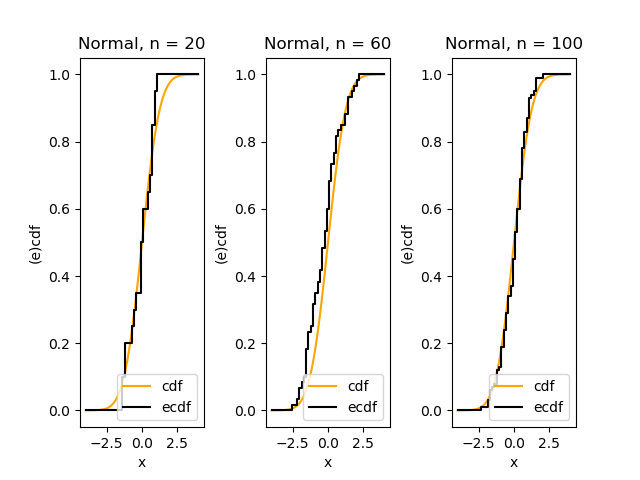
\includegraphics[width=\textwidth, height =0.4\textheight]{img/NormalCDF.png}
	\caption{Нормальное распределение}
	\label{fig:normal_cdf}
\end{figure}

\begin{figure}[H]
	\centering
	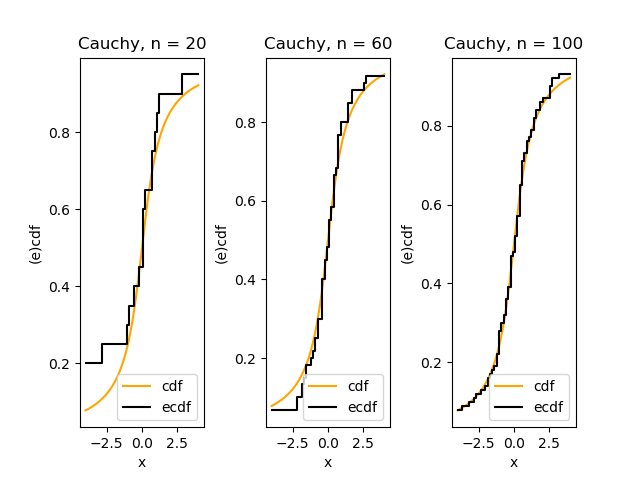
\includegraphics[width=\textwidth, height =0.4\textheight]{img/CauchyCDF.png}
	\caption{Распределение Коши}
	\label{fig:cauchy_cdf}
\end{figure}


\begin{figure}[H]
	\centering
	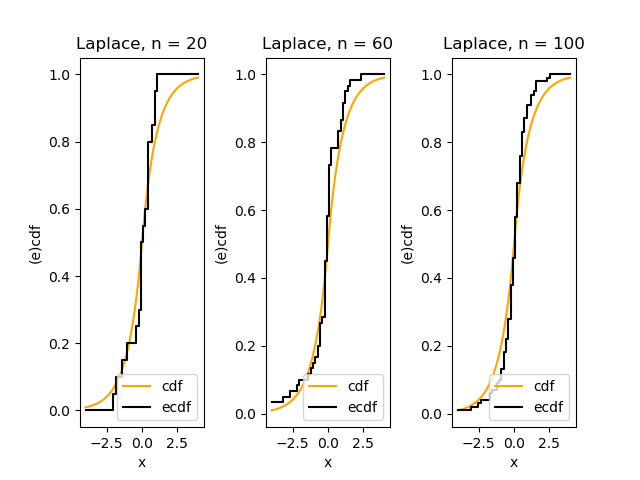
\includegraphics[width=\textwidth, height =0.4\textheight]{img/LaplaceCDF.png}
	\caption{Распределение Лапласа}
	\label{fig:laplace_cdf}
\end{figure}


\begin{figure}[H]
	\centering
	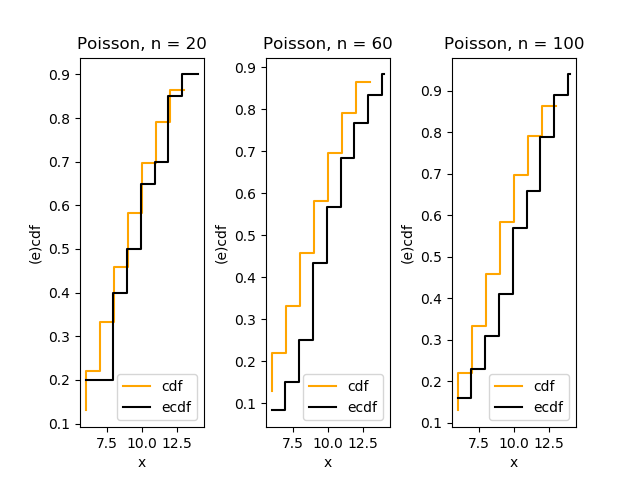
\includegraphics[width=\textwidth, height =0.4\textheight]{img/PoissonCDF.png}
	\caption{Распределение Пуассона}
	\label{fig:poisson_cdf}
\end{figure}


\begin{figure}[H]
	\centering
	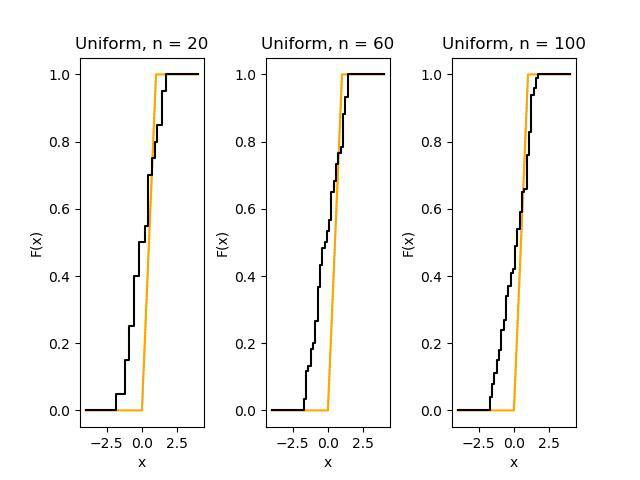
\includegraphics[width=\textwidth, height =0.4\textheight]{img/UniformCDF.png}
	\caption{Равномерное распределение}
	\label{fig:uniform_cdf}
\end{figure}

\subsection{Ядерные оценки плотности распределения}
\begin{figure}[H]
	\centering
	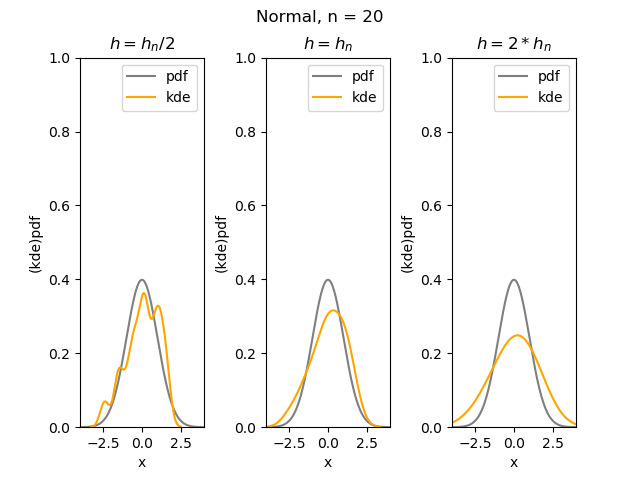
\includegraphics[width=\textwidth, height =0.4\textheight]{img/NormalKDE n = 20.png}
	\caption{Нормальное распределение, n = 20}
	\label{fig:normal_kde_20}
\end{figure}

\begin{figure}[H]
	\centering
	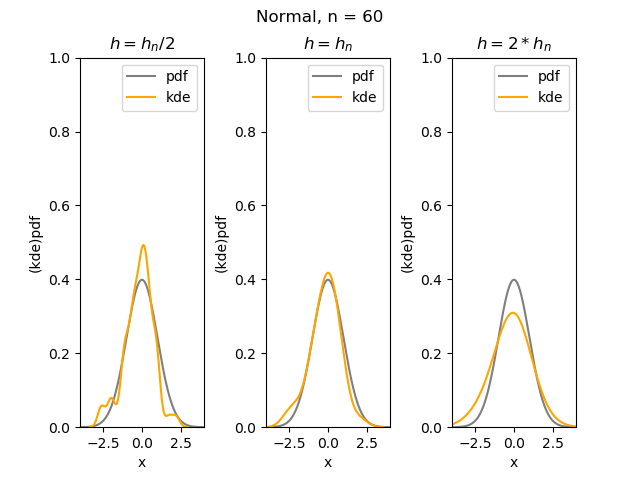
\includegraphics[width=\textwidth, height =0.4\textheight]{img/NormalKDE n = 60.png}
	\caption{Нормальное распределение, n = 60}
	\label{fig:normal_kde_60}
\end{figure}

\begin{figure}[H]
	\centering
	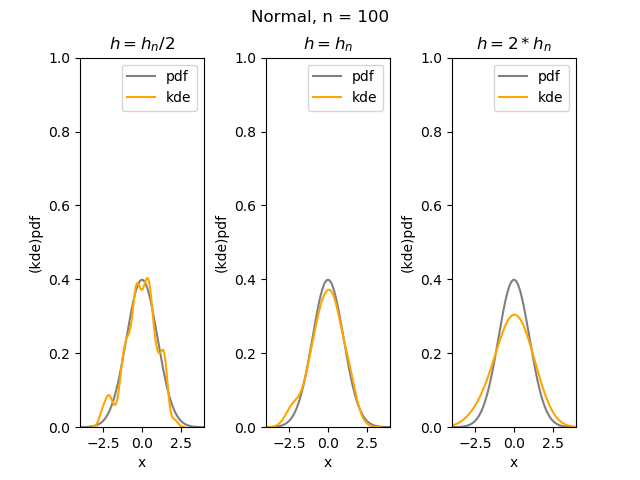
\includegraphics[width=\textwidth, height =0.4\textheight]{img/NormalKDE n = 100.png}
	\caption{Нормальное распределение, n = 100}
	\label{fig:normal_kde_100}
\end{figure}

\begin{figure}[H]
	\centering
	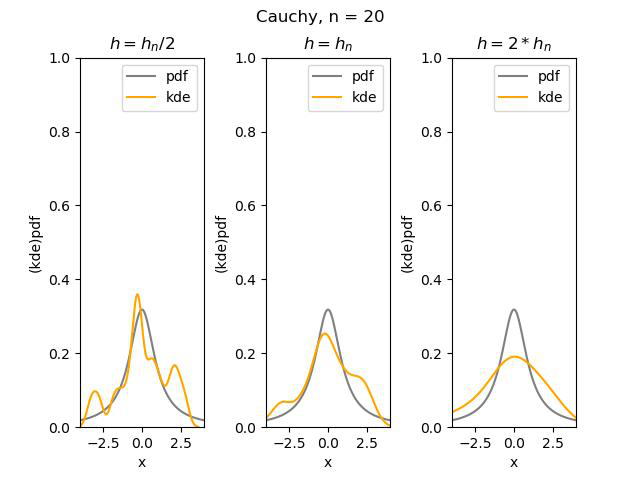
\includegraphics[width=\textwidth, height =0.4\textheight]{img/CauchyKDE n = 20.png}
	\caption{Распределение Коши, n = 20}
	\label{fig:cauchy_kde_20}
\end{figure}

\begin{figure}[H]
	\centering
	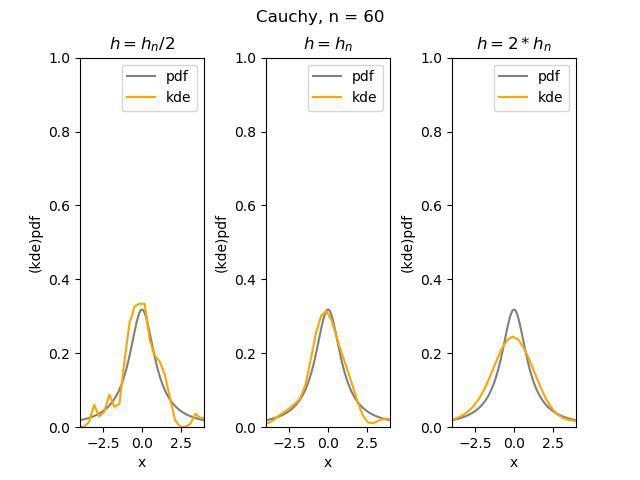
\includegraphics[width=\textwidth, height =0.4\textheight]{img/CauchyKDE n = 60.png}
	\caption{Распределение Коши, n = 60}
	\label{fig:cauchy_kde_60}
\end{figure}

\begin{figure}[H]
	\centering
	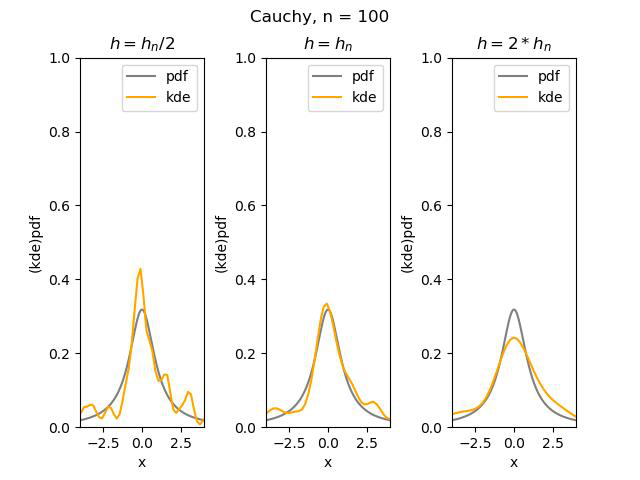
\includegraphics[width=\textwidth, height =0.4\textheight]{img/CauchyKDE n = 100.png}
	\caption{Распределение Коши, n = 100}
	\label{fig:cauchy_kde_100}
\end{figure}

\begin{figure}[H]
	\centering
	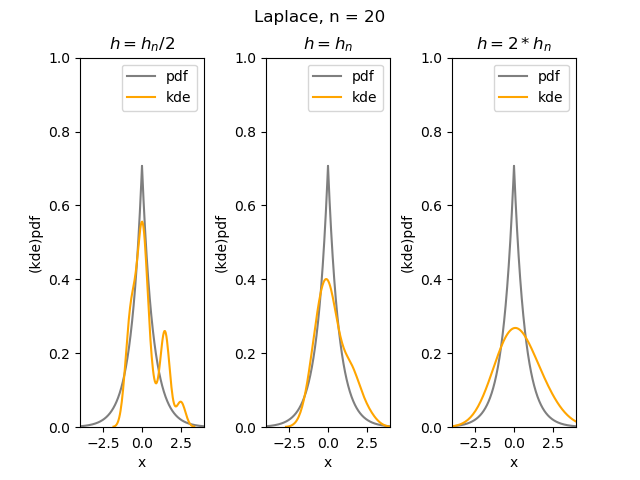
\includegraphics[width=\textwidth, height =0.4\textheight]{img/LaplaceKDE n = 20.png}
	\caption{Распределение Лапласа, n = 20}
	\label{fig:laplace_kde_20}
\end{figure}

\begin{figure}[H]
	\centering
	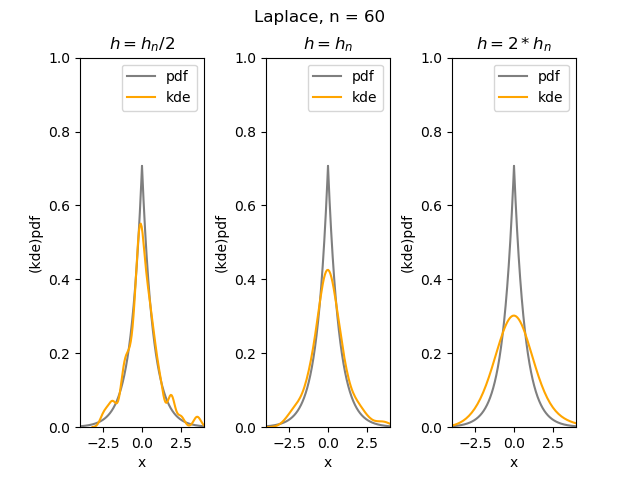
\includegraphics[width=\textwidth, height =0.4\textheight]{img/LaplaceKDE n = 60.png}
	\caption{Распределение Лапласа, n = 60}
	\label{fig:laplace_kde_60}
\end{figure}

\begin{figure}[H]
	\centering
	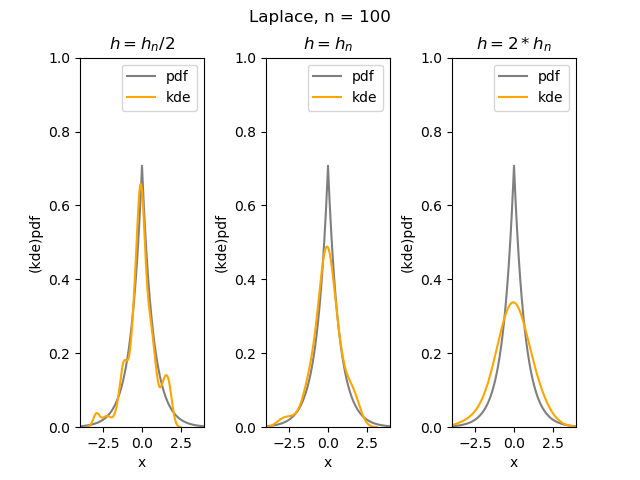
\includegraphics[width=\textwidth, height =0.4\textheight]{img/LaplaceKDE n = 100.png}
	\caption{Распределение Лапласа, n = 100}
	\label{fig:laplace_kde_100}
\end{figure}


\begin{figure}[H]
	\centering
	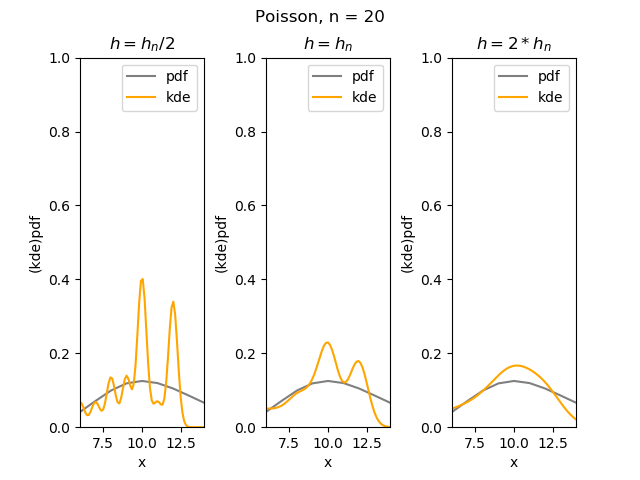
\includegraphics[width=\textwidth, height =0.4\textheight]{img/PoissonKDE n = 20.png}
	\caption{Распределение Пуассона, n = 20}
	\label{fig:poisson_kde_20}
\end{figure}

\begin{figure}[H]
	\centering
	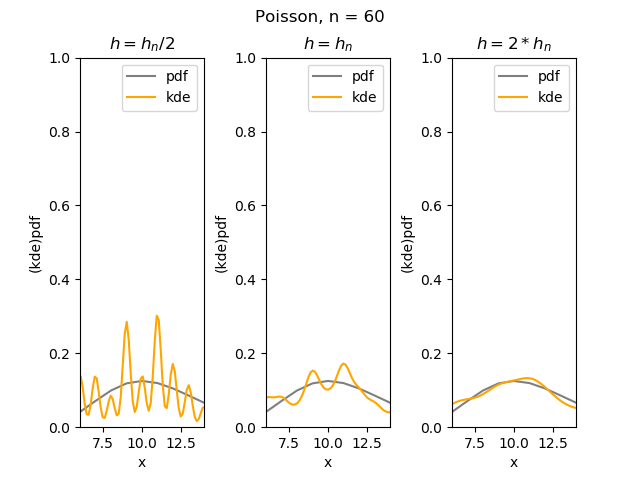
\includegraphics[width=\textwidth, height =0.4\textheight]{img/PoissonKDE n = 60.png}
	\caption{Распределение Пуассона, n = 60}
	\label{fig:poisson_kde_60}
\end{figure}

\begin{figure}[H]
	\centering
	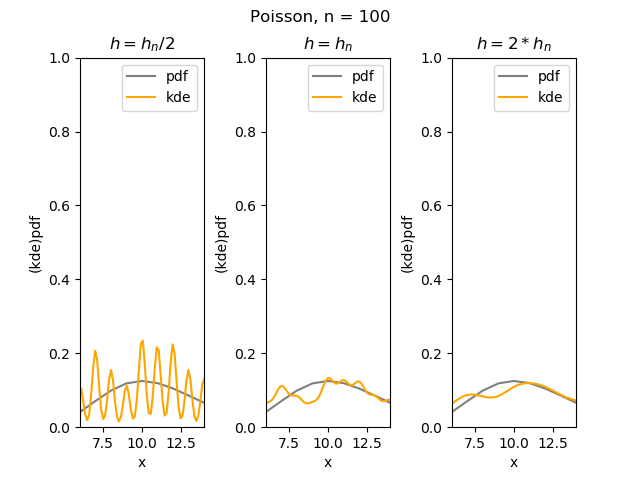
\includegraphics[width=\textwidth, height =0.4\textheight]{img/PoissonKDE n = 100.png}
	\caption{Распределение Пуассона, n = 100}
	\label{fig:poisson_kde_100}
\end{figure}


\begin{figure}[H]
	\centering
	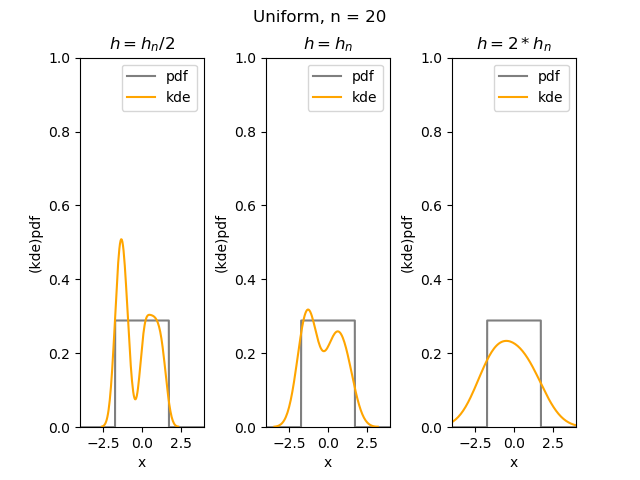
\includegraphics[width=\textwidth, height =0.4\textheight]{img/UniformKDE n = 20.png}
	\caption{Равномерное распределение, n = 20}
	\label{fig:uniform_kde_20}
\end{figure}

\begin{figure}[H]
	\centering
	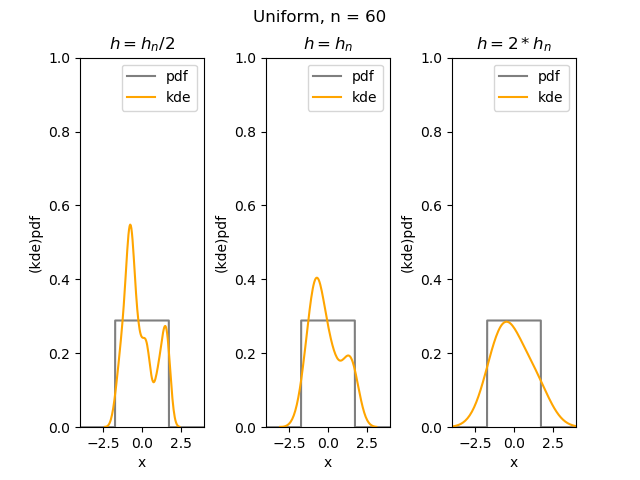
\includegraphics[width=\textwidth, height =0.4\textheight]{img/UniformKDE n = 60.png}
	\caption{Равномерное распределение, n = 60}
	\label{fig:uniform_kde_60}
\end{figure}

\begin{figure}[H]
	\centering
	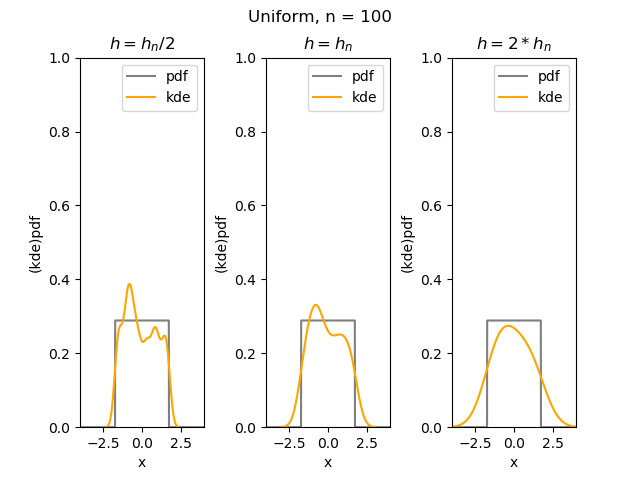
\includegraphics[width=\textwidth, height =0.4\textheight]{img/UniformKDE n = 100.png}
	\caption{Равномерное распределение, n = 100}
	\label{fig:uniform_kde_100}
\end{figure}

\end{document}